\chapter{Planning}
\label{Planning}
Dit hoofdstuk is het het laatste hoofdstuk van het tussentijds verslag. Het omschrijft de planning voor de komende maanden. 

Figuur \ref{imgGant} toon een grafische weergave van de planning in de vorm van een Gantt kaart. 

\begin{figure}[hpb]
	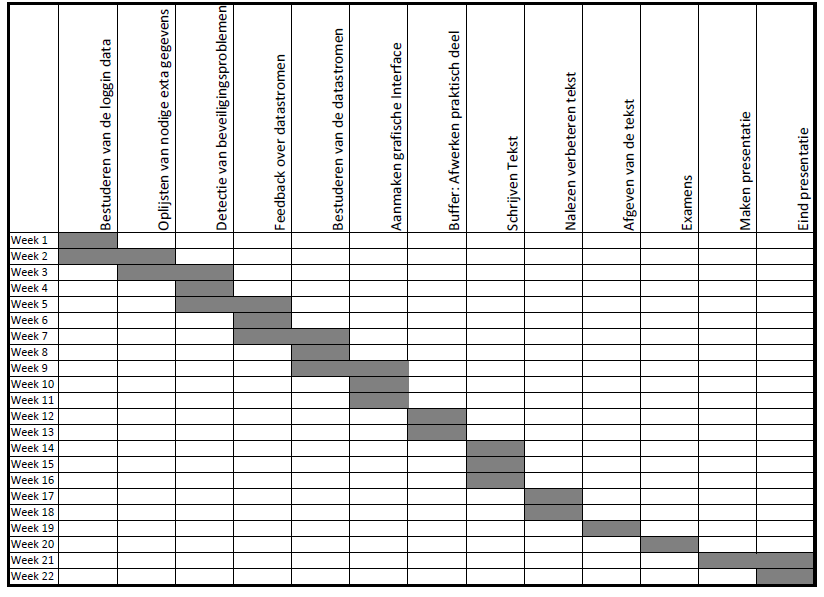
\includegraphics[scale=0.95]{Gantt.png}
	\caption{Gantt Shart}
	\label{imgGant}
\end{figure} 

Hierbij is week 1 de week van 15 tot en met 21 januari. Week 22 is de week van 24 juni. Naar schatting vallen daar ongeveer de masterproef verdedigingen. 
Er is een periode van drie weken voorzien om de tekst te schrijven. Natuurljk is dit niet voldoende. De tekst wordt tussendoor ook geschreven. Deze drie weken is voor het afronden van de tekst. 
